\section{Progressos}

Como foi especificado no documento de especifica��o, n�s seguiremos a arquitetura indicada na figura~\ref{arquitetura:global} abaixo.

\begin{figure}[h]%
\begin{center}
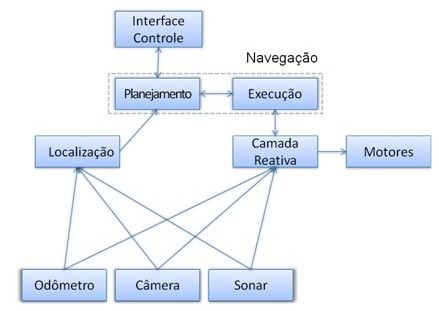
\includegraphics[width=.5\columnwidth]{imagens/arquitetura.jpg}
\caption{Arquitetura do Sistema completo.}%
\label{arquitetura:global}%
\end{center}
\end{figure}

Od�metros e sonares s�o sensores presentes na plataforma-rob� Pionner P2DX. A Vis�o ser� provida por uma c�mera comercial de baixo custo. Nossos testes est�o sendo realizados com a HS988 da Raysun Shine e com a Microsoft LifeCam VX1000.

Nossos progressos concentraram-se no M�dulo de Localiza��o, cuja arquitetura se baseia no uso do estimador bayesiano conhecido por Filtro Estendido de Kalman. A arquitetura detalhada do M�dulo de Localiza��o encontra-se na figura~\ref{arquitetura:localizacao} abaixo.

\begin{figure}[h]%
\begin{center}
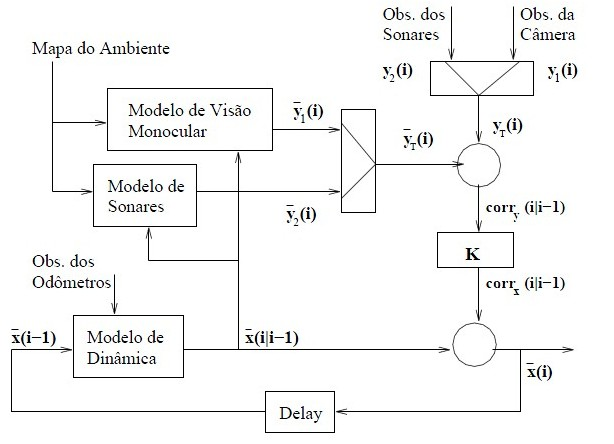
\includegraphics[width=.5\columnwidth]{imagens/arquitetura_localizacao.jpg}
\caption{Arquitetura Detalhada do M�dulo de Localiza��o.\cite{barra}}%
\label{arquitetura:localizacao}%
\end{center}
\end{figure}

Os trabalhos do �ltimo m�s resultaram em um avan�o consider�vel no m�dulo de localiza��o.

\subsection{Arquitetura do Sistema}
Todos os m�dulos do sistema foram integrados, e os testes do sistema completo come�aram. Uma arquitetura de software fortemente ass�ncrona e desacoplada foi desenvolvida, com resultados satisfat�rios. A arquitetura do sistema � descrita na se��o \ref{sec:arquitetura}.

\subsection{Filtro Estendido de Kalman (EKF)}
O c�digo do filtro estendido de Kalman, EKF, foi implementado e testado no simulador.

\subsection{Modelo de Din�mica}
O modelo de din�mica foi finalizado e testado no simulador. Ele � descrito na se��o \ref{sec:dinamica}.

\subsection{Modelo de Sonares}
O modelo de sonares foi finalizado e testado no simulador. Muito esfor�o foi gasto para garantir que a modelagem matem�tica dos sonares estava correta. As equa��es finais podem ser vistas na se��o \ref{sec:sonar}.

\subsection{Modelo de Vis�o}
Se��o \ref{sec:visao}.